% this file is called up by thesis.tex
% content in this file will be fed into the main document

%: ----------------------- name of chapter  -------------------------
\chapter{Conclusion} % top level followed by section, subsection


%: ----------------------- paths to graphics ------------------------

% change according to folder and file names
\ifpdf
    \graphicspath{{X/figures/PNG/}{X/figures/PDF/}{X/figures/}}
\else
    \graphicspath{{X/figures/EPS/}{X/figures/}}
\fi

%: ----------------------- contents from here ------------------------

\section{Future Work}

This paper discusses various issues regarding the development of 
The HCMP Player. The HCMP Player itself is part of a larger HCMP project 
that facilitates music representation, preparation, and performance.
There are some components that can be built upon the HCMP Player and some 
what can be directly integrated with the HCMP Player. Two
features can be added to further extend the HCMP Player's functionality. 

\subsection{Integrate with Score Following}
HCMP has a score following component which is also developed with Serpent.
Figure 7.1 is a screenshot of the score following component. The score 
following component can be used to notate a music score, turn
``pages''. The original score following component has a built-in player function,
and it can easily be replaced by the HCMP Player. With a set of predefined API 
of HCMP Player, score following components can be easily extended to coperate with 
the HCMP Player. The HCMP Player will synchronize with score following components 
by constantly receiving commands through the network. 

\begin{figure}[H]
\center{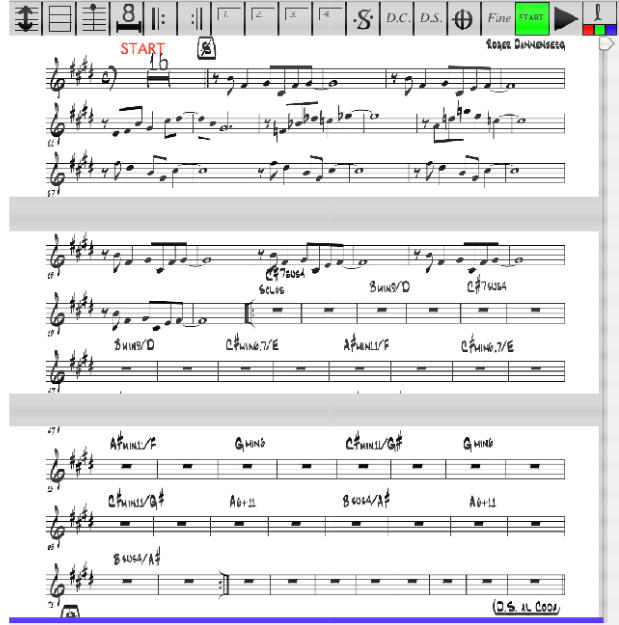
\includegraphics[width=0.5\linewidth]{8/1.png}}
\caption{HCMP Score Display Component}
\label{fig:speciation}
\end{figure}

\subsection{Integrate with Midi Database}
Another interesting work is about MIDI Database\cite{Dawen:ISMIR2011} which 
is based on Dawen Liang's previous work. The basic idea of MIDI Database 
is to create a tool by which a user is able to quickly record, organize
and retrieve audio information from various sources. The MIDI Database 
defines a complete set of API's for its clients. One possible extention of HCMP 
Player is to integrate MIDI Database into the HMCP Player library functions, 
so that users can easily use the HCMP Player to search and play MIDI 
segements from a previous history Database.

\section{Conclusion}
From the HCMP project's perspective, the HCMP Player is a building block for a 
larger project upon which more powerful components can be built. It can also 
coperate with other components to complete a complex job, or be used by other
components. From a developer's 
perspective, the HCMP Player provides a complete set of API's which can be extended 
and tailored to fit into a more sophisticated project.
The HCMP Player can be split into 3 parts:  
GUI, player engine and network. The design and usage of each part 
is explained in detail in the previous chapters. I also briefly decribe 
the implementation of each part. As a supplementary,
some pseucode segments are provided to illustrate logic. A complete list of
the HCMP Player features is provides and a successful criteria is defined to
help evaluate the project.
